\chapter{Theoretische Grundlagen}
\label{ch:grundlagen}

\section{Relevanz}

Relevanz ist allgemein beschrieben eine Beziehung zwischen einem Individuum, dem zeitlichen Rahmen, in welchem dieses eine Information benötigt und einer beliebigen Information.\footnote{Vgl. Bookstein S. 1 \cite{bookstein2007}}
Das bedeutet, dass Relevanz von Person zu Person unterschiedlich ist, da zum einen diverse Informationen nur zu einer bestimmten Zeit notwendig bzw. wichtig sind und zum anderen der Kontext der benötigten Information sich ständig ändert.

Um zu verstehen, woher die Relevanz stammt bzw. in der Informationstechnik verwendet wird, ist es wichtig, die Gewinnung von Informationen aus Objekten (\emph{Information Retrieval}) zu verstehen.
Dieser Teil der Wissenschaft beschäftigt sich mit dem präzisen Abruf von Informationen, um das Informationsbedürfnis (\emph{Information need}) eines Nutzers zu stillen.
Dieses Informationsbedürfnis wird von einem idealen Suchobjekt befriedigt, stellt also die Spezifikation eines idealen Objekts dar.
Diese Spezifikation geht über den reinen textuellen Inhalt der Suche hinaus und umfasst auch kontextuelle, zeitliche und andere Aspekte.
Die Bestimmung der Relevanz ist dabei die Aktivität bzw. Praxis um diesen idealen Inhalt zu finden.\footnote{Vgl. Manning, Raghavan, Schütze \cite{manning2008}}

Im Falle von Crossload ist das ideale Objekt beispielsweise eine bestimmte Predigt, die zu einem bestimmten Zeitpunkt in einer bestimmten Kirche gehalten wurde oder ein Bild, welches zu einer gewissen Bibelstelle gehört.
Im Beispiel Google, ist das Objekt eine bestimmte Webseite, die zu einem bestimmten Suchbegriff passt.
Aufgabe von Suchmaschinen ist es, die Relevanz zwischen dem Suchbegriff und dem Objekt zu bestimmen und dem Nutzer die Objekte anzuzeigen, die dem Suchbegriff am nächsten kommen.

\section{Methoden zur Bewertung von Relevanz}

Eine \gls{searchEngine} gibt nach einer Suchanfrage Ergebnisse standardmäßig sortiert nach der Relevanz der Ergebnisse abhängig zum gegebenen Suchbegriff des Nutzers zurück.
Die Schwierigkeit dabei ist die Bestimmung der Relevanz für eine beliebige Website.
Die dafür genutzten Funktionen und Methoden werden allerdings von den Unternehmen geheim gehalten, um einen Missbrauch ihrer \gls{searchEngine} zu verhindern.
Dennoch sind die am häufigsten genutzten Merkmale bekannt und in einigen wissenschaftlichen Arbeiten untersucht worden.\footnote{Vgl. Zaragoza, Najork, S. 1 \cite{zaragoza2018}}
Moderne Suchmaschinen nutzen dutzende oder gar hunderte verschiedener Methoden und Features um die Relevanz der verfügbaren Suchergebnisse zu bewerten, wird im Folgenden nur auf einige bekannte Methoden eingegangen.

Bei der Webapplikation \gls{crossload} handelt es sich um eine Internetsuche, welche beispielsweise mit Google, Bing, Ecosia oder anderen \gls{searchEngine}n üblich ist.
Deren grundlegende untersuchte Funktionalität, die Suche und Bestimmung der Relevanz, ist vergleichbar.
Unterschiedlich sind sie in der Art der Ergebnisse (Google sucht nach Webseiten, Crossload nach Predigten, Bilder, etc.) und der Menge an untersuchten Ergebnissen.
Aus diesem Grund werden nachgehend Methoden zur Bewertung der Relevanz von Informationen aus Webseiten betrachtet.

\subsection{Textuelle Relevanz}
\label{sub:relevanceText}
Das einfachste Merkmal für die Bewertung der Relevanz ist den kompletten Inhalt nach der textuellen Relevanz zu bewerten.
Da natürliche Sprache, die meist für Suchergebnisse genutzt wird, generell ungenau ist, wird mit sogenannten „Matching Functions“ versucht auch ungefähre Übereinstimmungen in einem Fließtext zu finden.
Einige der verwendeten Funktionen um die textuelle Relevanz zu bewerten sind dabei:\footnote{Vgl. Zaragoza, Najork, S. 1 \cite{zaragoza2018}}

\begin{itemize}
  \item Die Anzahl der Treffer für den Suchterm oder Abwandlungen
  \item Position des Suchterms (früheres Vorkommen, z. B. im Titel)
  \item Seitenstruktur (für Webseiten: Ist der Term eine Überschrift o. ä.)
  \item Grafisches Layout (für Webseiten: Ist der Term z. B. farblich markiert)
  \item Levenshtein Distanz\footnote{Vgl. Levensthein \cite{levenshtein1966binary}} (die minimale Anzahl an Operationen, um eine Zeichenkette in eine andere umzuwandeln)
\end{itemize}

\subsection{Relevanz durch Attribute}
\label{sub:relevanceAttribute}
Des Weiteren ist es auch möglich den durchsuchten Objekten Attribute zuzuweisen, um für Schlagwörter relevantere Ergebnisse zu erlangen.
Diese können entweder von Nutzern selbst bestimmt werden, wie z. B. bei der Website Flickr\footnote{Vgl. Liu et.al., S. 1-3 \cite{liu2009}}, um Bilder für bestimmte Themen höher werten zu lassen oder werden von Algorithmen aufgrund von Bilderkennung automatisch zugewiesen.

Ein Beispiel hierfür ist Google, welches eine frei verwendbare Machine Learning API\footnote{Vgl. Google ML Dokumentation \cite{googledevelopers2022}} oder eine direkte Integration, in die Google Fotos App anbietet. Diese Anwendung teilt automatisch die gemachten Bilder in verschiedene Kategorien ein.\footnote{Vgl. Google Fotos \cite{googlephotos2022}}

Möglich gefundene Ergebnisse können auch durch Existenz oder Nichtvorhandensein eines Attributs höher gewichtet werden.
Dadurch können zum Beispiel bereits aufbereitete Ergebnisse eine höhere Relevanz erhalten. \footnote{Siehe Crossload Search API \cite{crossload2022}}

\subsection{Hyperlink Relevanz}
\label{sub:relevanceHyperlink}
Für Suchergebnisse im Internet oder andere miteinander verlinkte Seiten, wie z. B. in internen Dokumentationsseiten, Wikis o. ä., können auch die Hyperlinks genutzt werden, um die Relevanz eines Ergebnisses zu bestimmen.
Ein Hyperlink besteht hierbei aus dem angezeigten Text auf der Quellseite und einem Link zur Zielseite oder auf einen bestimmten Abschnitt dergleichen.
Hyperlinks werden aber nicht von einer Maschine in eine Seite eingefügt, sondern jeder Link wird von Menschen gesetzt.
Aus diesem Grund kann man hier von „menschlicher Intelligenz“ sprechen.\footnote{Vgl. Zaragoza, Najork, S. 2 \cite{zaragoza2018}}

Um einen Treffer höher zu gewichten, ist eine Option die Anzahl an Verlinkungen auf eine Seite zu zählen und absteigend zu sortieren.\footnote{Vgl. Marchiori \cite{marchiori1997}}
Alternativ kann der angezeigte Linktext noch zusätzlich als eine Art Attribut (\ref{sub:relevanceAttribute}) oder erweiterte textuelle Referenz (\ref{sub:relevanceText}) gesehen werden, der dann bei der Auswertung einer Suche mitverwendet wird.\footnote{Vgl. Page, Brin, Motwani und Winograd \cite{ilprints422}}

\subsection{Relevanz durch Nutzerverhalten}
\label{sub:relevanceUser}
Um unabhängiger von manuellem Verlinken zwischen Seiten zu werden, haben bekannte Suchmaschinen auch Möglichkeiten entwickelt, die Anzahl der „erfolgreich“ gefundenen Treffer zu zählen und als relevanter zu gewichten.
Im Umfeld einer Internetsuche wäre der „erfolgreich“ gefundene Treffer ein Klick auf die entsprechende Website.
Diese können entweder live oder durch Auswertung von Log Dateien analysiert werden.
Andere Wege um die Anzahl an Besuchen auf einer Website zu messen, umfassen Tracking Methoden, Toolbars oder Werbung.
Die Bewertung der Relevanz durch das untersuchte Nutzerverhalten ist überaus erfolgreich, da hier von einer Art Schwarmintelligenz ausgegangen wird, die Nutzern für die gleiche Suche Ergebnisse anzeigt, die schon viele Benutzer davor angeklickt haben.\footnote{Vgl. Joachims, Radlinski, S. 1 \cite{joachims2007}}

\subsection{Performance}
\label{sub:relevancePerformance}
Da Suchmaschinen dem Nutzer eine bestmögliche Benutzererfahrung, auch bekannt als User Experience, ermöglichen wollen, sollen die gefundenen Webseiten dies bieten. Eine Möglichkeit dies zu messen, ist die Performance einer Website.
Die Performance einer Webseite oder eines Suchergebnisses umfasst die Ladegeschwindigkeit, Speicherverbrauch und benötigte Leistung um das Ergebnis komplett anzuzeigen.
Da dies nicht für x-Millionen Treffer bei jeder Suchanfrage getestet werden kann, werden mögliche Suchtreffer vorher indiziert und nach der Performance untersucht.
Dadurch entsteht ein Performance-Score, welcher dann für die Relevanz verwendet werden kann.\footnote{Vgl. Manning, Raghavan, Schütze \cite{manning2008}}

Im aktuellen Beispiel von Crossload, ist die Performance eines Suchergebnisses durch die Anzahl an gefundenen Treffern und die Anzahl an gefundenen Treffern mit einem bestimmten Attribut, wie z. B. „Performance: 5“ oder „Performance: 4“, definiert.

\clearpage
\section{Auswertung der Relevanz von Suchergebnissen}
\label{sec:relevanceScore}
Um letztendlich Ergebnisse mit der höchsten Relevanz zu erhalten, wird meist eine Kombination aus mehreren der o.g. Methoden benutzt, um die komplette Relevanz für einen Treffer zu bewerten.
Die Herausforderung dabei ist die genaue Gewichtung der einzelnen Methoden, um die Relevanz eines Treffers optimal zu bewerten.
Für jeden Treffer wird dann ein Relevanzscore berechnet, der sich aus den einzelnen Methoden zusammensetzt. Nach diesem Score wird in einer Liste absteigend sortiert, um das relevanteste Ergebnis als erstes Element zu erhalten.

Sollte sich der Score eines Treffers in der Relation zu anderen Wertungen weit absetzen, kann dieser Treffer dem Nutzer auch direkt vorgeschlagen werden.\footnote{Vgl. Turnbull, Berryman, S. 225-228 \cite{turnbull2016}}
Dieser Vorschlag kann anschließend hervorgehoben werden, um dem Nutzer die Entscheidung zu erleichtern. Damit der Vorschlag für den Nutzer sichtbar ist, wird der Vorschlag in der Liste der Suchergebnisse grafisch hervorgehoben, oder es wird ein separater Abschnitt für den Vorschlag angezeigt.
Dies wird von \gls{searchEngine}n wie Google, Bing oder Ecosia bereits verwendet.
Diese \gls{searchEngine}n präsentieren dem Nutzer ein ideales Ergebnis meist an der Seite der restlichen gefundenen Treffer.\footnote{Vgl. Google \cite{google2022}, Bing \cite{bing2022}, Ecosia \cite{ecosia2022}}

\begin{figure}[h]
  \begin{centering}
    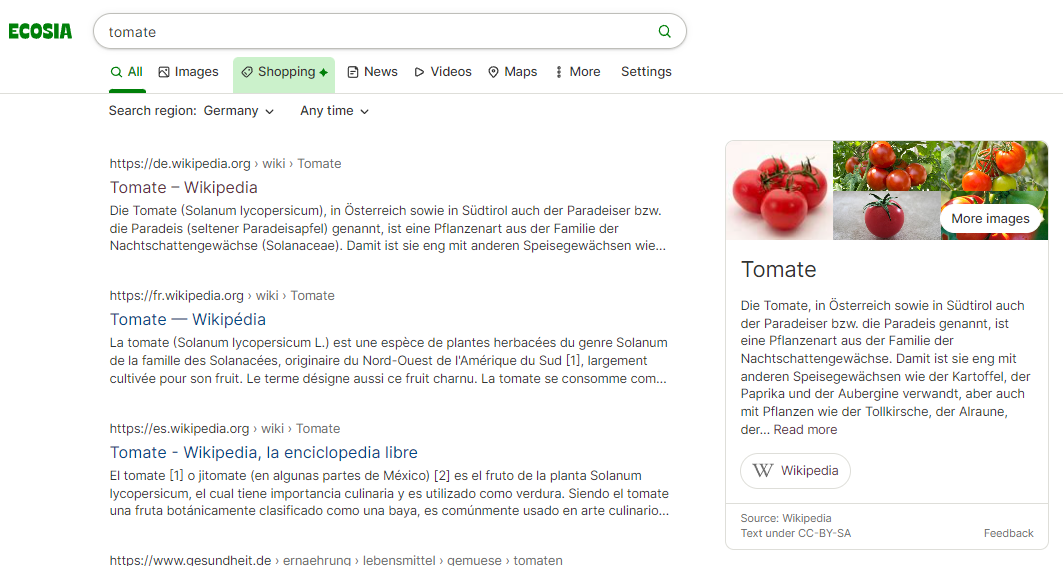
\includegraphics[width=\textwidth]{figures/foundations/tomato.png}
    \caption{Vorschlag eines Wikipedia Artikels zum Thema Tomate \cite{ecosia2022}.}
    \label{fig:tomate}
  \end{centering}
\end{figure}

\clearpage
Dieses Vorschlagen von Ergebnissen kann auch verwendet werden, um bereits bei der Eingabe einer Abfrage durch Autovervollständigung (eng. „Search Completion“) geschehen.\footnote{Vgl. Turnbull, Berryman, S. 206-218 \cite{turnbull2016}}
Der Unterschied ist hierbei der angezeigte Ort, an dem die Vorschläge erfolgen.
Für den Suchvorschlag wird er direkt in der Suchleiste angezeigt, während der Vorschlag eines Treffers in der Ergebnisliste erfolgt.

\begin{figure}[h]
  \begin{centering}
    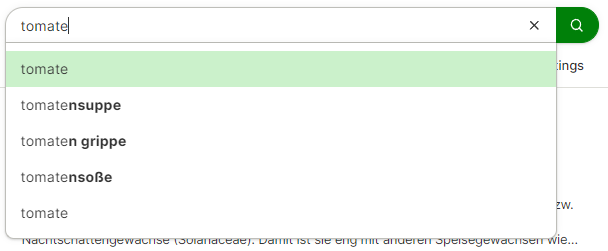
\includegraphics[width=\textwidth]{figures/foundations/tomatoSuggestion.png}
    \caption{Vorschlag von Suchbegriffen zum Thema Tomate \cite{ecosia2022}.}
    \label{fig:tomateVorschlag}
  \end{centering}
\end{figure}

Für kleinere Anwendungen ist hierbei meist ein manuelles Einstellen nach einem \gls{trialAndError} Verfahren notwendig, bei denen einige wenige Methoden unterschiedlich gewichtet werden.
Dies wird dann von Zeit zu Zeit wiederholt, wenn neue Erkenntnisse aus Tests oder dem produktiven Betrieb zurückkommen.\footnote{Vgl. Zaragoza, Najork, S. 3 \cite{zaragoza2018}}
Große Suchmaschinen nutzen hierfür allerdings, wie bereits erwähnt, hunderte Methoden und evaluieren deren Erfolg im produktiven Betrieb durch proprietäre statistische Methoden.\footnote{Vgl. Taylor, Zaragoza, Craswell, Robertson, Burges \cite{taylor2006}}

\chapter{Technische Grundlagen}
\label{ch:technischeGrundlagen}
\section{Apache Lucene}
\label{sec:lucene}

Apache Lucene, oder auch kurz Lucene genannt, ist eine mächtige Suchbibliothek, die plattformunabhängig von verschiedenen bekannten Apps, wie z. B. Netflix eingesetzt wird.
Sie nutzt für die Indizierung zu durchsuchender Dokumente Textfelder, wie z. B. „title“ für den Titel eines Dokumentes, um sowohl den Inhalt als Volltext, als auch die Attribute durchsuchen zu können. \footnote{Siehe Apache Lucene \cite{lucene2022}}
Lucene stellt dabei folgende Funktionen bereit:\footnote{Vgl. Schindler, Bräuer, Diepenbroek, S.4 \cite{schindler2007}}
\begin{itemize}
  \item \textbf{Sortierte Suche:} die besten Ergebnisse werden zuerst bezeigt
  \item \textbf{Leistungsstarke Queries:} Phrasenabfragen, Platzhalterabfragen („wildcards“), Abfragen zur Nähe bzw. Ähnlichkeit eines Suchergebnisses („promixmity search“), exakte Phrasenabfragen, Bereichsabfragen für Datum/Uhrzeit und Zahlen
  \item \textbf{Feldbasierte Suche:} Alle oder bestimmte Felder durchsuchen
  \item \textbf{Boolesche Operatoren:} Beliebige Kombinationen zwischen Suchbegriffen (AND, OR,
  NOT) um einzelne Abfragen zu kombinieren.
  \item \textbf{Sortieren nach einem beliebigen Feld}
\end{itemize}

\section{Apache Solr}
\label{sec:Solr}
Solr ist von Crossload verwendete Such Engine, die als Web Schnittstelle dient, um auf einer Datenmenge Suchanfragen mit Apache \gls{lucene} auszuwerten.\footnote{Siehe Apache Solr \cite{solr2022}}

Solr benutzt hier die Indexing Funktionen von Lucene, um in Echtzeit alle verfügbaren Dokumente zu indizieren, um bei einer Suche nur den Index durchsuchen zu müssen.
Mit Apache Zookeeper wird dann eine \gls{api} zur Verfügung gestellt, welche Synchronisierung, Namensregister und die Verteilung der Konfiguration bereitstellt.
Inhalte werden anhand von Boostingmechanismen höher oder schlechter bewertet.
Als Entwickler gibt man hierfür mögliche Textfelder an, auf denen Solr automatisch ein Textmatching anwendet.\footnote{Vgl. \ref{sub:relevanceText}}
Die wichtigsten Features von Solr sind:\footnote{Siehe Apache Solr \cite{solr2022}}
\begin{itemize}
  \item Volltextsuche
  \item Facettensuche (generierte Attribute)
  \item Suchvorschläge und Autokorrektur
  \item Echtzeit Indizierung des Suchergebnisindizes
  \item Arbeiten mit Word und PDF Dokumenten
  \item Erstellung eigener Boostingmechanismen (z. B. mit Java)
\end{itemize}

\chapter{Crossload}
\label{ch:Crossload}

\section{Einführung}
\label{sec:crossload}

Crossload ist eine deutsche Predigtdatenbank, deren Ziel es ist, mit modernen Technologien und einem ansprechendem User Interface (\gls{ui}) den Zugang zu Predigten und anderem christlichen Material zu vereinfachen.
Hierzu werden teils Predigten aus anderen System importiert, teils Autoren angefragt, welche dann regelmäßig ihre eigenen Predigten selbstständig hochladen.
Dadurch sind sowohl ältere Predigten, etwa von Martin Luther, als auch Predigten zu aktuellen Themen und Weltgeschehen verfügbar.
Zudem gibt es Schnittstellen zu christlichen Verlagen oder Webseiten wie CLV\footnote{Siehe CLV \cite{clv2022}} oder Evangelium 21\footnote{Siehe Evangelium 21 \cite{evangelium21e.v.2022}}.\footnote{Vgl. Pfleiderer, Crossload \cite{pfleiderer2022}}
Auf Crossload gibt es derzeit Predigten mit und ohne Video, Bücher, Bilder, Musik, Hörbücher und andere bzw. noch nicht kategorisierte Inhalte.

\section{Technische Architektur}
\label{sec:architektur}

Technisch ist Crossload wie folgt aufgestellt:
\begin{itemize}
  \item \textbf{Frontend:} UI entwickelt mit Angular zum Durchsuchen der Datenbank und direktem Streaming der Predigten. Für die Analyse und Statistiken wird \gls{matomo} verwendet. Dieser Dienst verfolgt besuchte Seiten, angehörte Inhalte und abgegebene Suchanfragen. Das Open-Source Pendant zu Google Analytics enthält auch Statistiken zur durchschnittlichen Dauer eines Besuches.\footnote{Siehe \gls{matomo} \cite{matomo2022}}
  \item \textbf{Backend/Suche:} Eine auf Solr basierte REST API mit allen veröffentlichten Inhalten und anderen Metadaten. Sie wird verwendet, um performante Suchanfragen des Frontends bearbeiten zu können und relevante Ergebnisse zu liefen.
  \item \textbf{Redaktion:} Aufbereitung und Anlegen von Inhalten verschiedenster Kategorien und anderer Metadaten.
  \begin{itemize}
    \item \textbf{Angular UI}: Redaktionelles Backend zum Pflegen aller Daten von Crossload.
    \item \textbf{Node.js RESTFUL API}: Schnittstelle zwischen der UI, der Datenbank und AWS.
    \item \textbf{\gls{aws}}: Speicherung von Dateien (Audio, Video, Bilder).
    \item \textbf{\gls{mongo}}: Datenbank zur Verwaltung und Speicherung aller Daten.
  \end{itemize}
\end{itemize}

\section{Suche bei Crossload}
\label{sec:implementedFunctionality}

Bei \gls{crossload} werden verschiedene Typen bzw. Kategorien von Inhalten in der von Solr indizierten Datenbank über eine Spring Boot Anwendung an das Webfrontend zur Verfügung gestellt.
Diese Inhalte werden anhand von eingegebenen Suchbegriffen, aktuellen Ereignissen oder Attributen wie Themen, Autoren oder Bibelstellen gefiltert.

Falls der Nutzer keine Suchanfrage eingegeben hat, werden die neuesten bzw. die aktuell relevantesten Inhalte angezeigt.
Diese Suche kann direkt über die Startseite erreicht werden, wenn man auf den Suchknopf (eine Lupe) klickt.
Sollte der Nutzer in das Suchfeld etwas eingegeben haben, wird die Suche direkt nach dem Klick auf die Lupe gestartet und er erhält Ergebnisse abhängig von seiner Eingabe.

\begin{figure}[h]
  \begin{centering}
    
\includegraphics[width=\textwidth]{figures/foundations/crossloadSucheStart.png}
    \caption{Startseite der Suche bei Crossload \cite{pfleiderer2022}.}
    \label{fig:crossloadSucheStart}
  \end{centering}
\end{figure}

Der initiale und derzeit implementierte Gedanke ist, die Inhalte auch in diesen Kategorien zu übertragen und in fester Reihenfolge anzuzeigen.
Diese Suchergebnisseite enthält pro Kategorie 5 Inhalte und einen Link, um alle Ergebnisse dieser Kategorie anzuzeigen.
Dadurch konnte bisher dem Nutzer ein schneller Einblick in die Inhalte gegeben werden, ohne dass er sich durch viele Ergebnisse klicken muss.
Die Kategorien sind hierbei nach der erwarteten Häufigkeit sortiert, in welcher die Entwicklung das Verhalten des Nutzers erwartet.

Diese Vorgehensweise hat jedoch einige Nachteile:

\begin{itemize}
  \item \textbf{Relevanz:} Der möglicherweise relevanteste Inhalt wird nicht als Erstes angezeigt, da dessen Kategorie relativ weit unten angezeigt wird.
  \item \textbf{Übersicht:} Es ist schwer für den Nutzer eine Übersicht über alle gefundenen Inhalte zu erlangen.
  \item \textbf{User Experience:} Höchstwahrscheinliche Treffer (90-100 \% Trefferwahrscheinlichkeit) werden nicht direkt vorgeschlagen.
  Ein Treffer ist hierbei sehr wahrscheinlich relevant, wenn er ein Treffer mit einem sehr hohen errechneten Relevanzscore ist.
\end{itemize}

Diese Nachteile sollen im Verlaufe der Entwicklung behoben werden.
Ebenso sollen auch die bisher genutzten Methoden zur Berechnung der Relevanz verbessert werden.
Diese umfassen derzeit:

\begin{itemize}
  \item Text Matching auf verschiedene Textteile und Attribute. Hier werden verschiedene Attribute in 3 Kategorien (hoch, mittel, niedrig) wie folgend bewertet:
  \begin{itemize}
    \item \textbf{Hoch:} Titel, Serie, Thema, Autor
    \item \textbf{Mittel:} Untertitel, Schlagwörter, Kategorie, Thema
    \item \textbf{Niedrig:} Verlag, Standort, Dateiname, Speech to Text, Mitschrift, Suchsnippet
  \end{itemize}
  \item Matching des Suchterms zu einem Bibelvers.
  \item Inhalte mit Video oder Bild werden höher bewertet, da diese qualitativ hochwertiger sind.
  \item Filter für mitgegebene Query Parameter: Kategorie, Serie, Event, Thema, Jahreszahl oder Dauer. Inhalte, die nicht zu diesem Filter passen, werden komplett aussortiert.
\end{itemize}
